\chapter{Introduction}
% \label{chap:intro}

% \section{Introduction}
\section{Motivations}
% \label{sec:motivation}
Sự bùng nổ của điện toán đám mây, đặc biệt là nền tảng Amazon Web Services (AWS), đã mang lại khả năng mở rộng và linh hoạt chưa từng có cho các doanh nghiệp. Tuy nhiên, đi kèm với lợi ích đó là sự gia tăng phức tạp trong việc quản lý hạ tầng và đảm bảo an ninh. Các công cụ đánh giá bảo mật đám mây (Cloud Security Posture Management - CSPM) hiện nay như Prowler hay ScoutSuite đóng vai trò quan trọng trong việc phát hiện các lỗ hổng cấu hình. Mặc dù rất mạnh mẽ trong việc chỉ ra các sai sót kỹ thuật, nhưng kết quả đầu ra của chúng thường dừng lại ở các báo cáo dạng văn bản hoặc dữ liệu thô (JSON, CSV). Điều này tạo ra một gánh nặng lớn cho các kỹ sư vận hành, khi họ phải thủ công phân tích từng cảnh báo, đối chiếu tài liệu và tự thực hiện các thao tác sửa lỗi (remediation) lặp đi lặp lại.

Trong khi đó, các Mô hình Ngôn ngữ Lớn (LLM) đã cho thấy khả năng vượt trội trong việc hiểu và xử lý ngôn ngữ tự nhiên. Tuy nhiên, nếu chỉ sử dụng LLM như một công cụ tư vấn (chatbot) thụ động thì chưa đủ để giải quyết bài toán vận hành thực tế, vì chúng thiếu khả năng tương tác trực tiếp với môi trường để thực thi hành động.

Để giải quyết khoảng cách giữa việc "phát hiện lỗi" và "xử lý lỗi", đồ án này đề xuất nghiên cứu và xây dựng một hệ thống Tác tử AI Tự hành (Autonomous AI Agent) dựa trên kiến trúc Đa tác tử (Multi-agent system) kết hợp với kỹ thuật Gọi công cụ (Tool Calling). Thay vì chỉ đưa ra lời khuyên, hệ thống này được thiết kế để hoạt động như một đội ngũ kỹ sư ảo, trong đó các tác tử chuyên biệt phối hợp với nhau để thực hiện nhiệm vụ. Điểm đột phá của phương pháp này nằm ở khả năng "Tool Calling" – cho phép LLM không chỉ sinh văn bản mà còn có thể ra quyết định gọi các lệnh thực thi (như AWS CLI, Prowler CLI) để thao tác trực tiếp trên hạ tầng đám mây.

Cách tiếp cận này cho phép hệ thống tự động hóa trọn vẹn quy trình đánh giá bảo mật: từ việc chủ động quét môi trường để phát hiện rủi ro, phân tích mức độ nghiêm trọng, cho đến việc tự động thực thi các hành động khắc phục (remediation) để vá lỗ hổng ngay lập tức mà không cần sự can thiệp thủ công của con người. Đây là bước tiến quan trọng nhằm chuyển đổi quy trình bảo mật từ mô hình thụ động sang mô hình chủ động và tự hành hoàn toàn.
\begin{figure}[H]
\vspace{2pt}
\centering
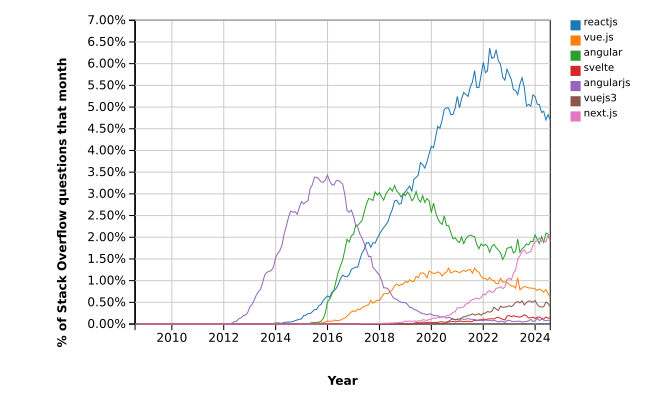
\includegraphics[width=1\textwidth]{Images/Introduction/stackoverflow-trends-chart.png}
\vspace{.1cm}
\caption{The popularity of frameworks based on StackOverflow questions 2008-2024}
\end{figure}

To illustrate, consider the Next.js framework, which has gained significant popularity in recent years. Built on top of React.js (currently the most popular front-end library), Next.js has seen rapid growth and frequent updates. For instance, version 13.0.0 of Next.js was released on October 25th, 2022, followed by multiple version 13.x.x updates, until version 14.0.0 was released on October 26th, 2023. Just 1 year later, they released version 15.0.0 for the framework with many breaking changes\footnote{\href{https://nextjs.org/blog}{The latest Next.js news - https://nextjs.org/blog}}. This rapid pace of development introduces challenges for developers who need to maintain or upgrade their codebases, especially considering that React.js itself has also undergone significant changes, such as the switch from version 18.0.0 to 19.0.0, which involved major updates\footnote{\href{https://react.dev/blog/2024/04/25/react-19-upgrade-guide}{How to Upgrade to React 18 - https://react.dev/blog/2024/04/25/react-19-upgrade-guide}}.

\section{Objectives}

Mục tiêu chính của nghiên cứu này là thiết kế và xây dựng một hệ thống Tác tử AI Tự hành (Autonomous AI Agent) có khả năng đánh giá, báo cáo và nâng cao mức độ trưởng thành về bảo mật trên nền tảng AWS. Bằng cách tận dụng kiến trúc \textbf{Đa tác tử (Multi-agent systems)} và kỹ thuật \textbf{Gọi công cụ (Tool Calling)}, đồ án hướng tới các mục tiêu cụ thể sau:

\begin{itemize}
  \item Xây dựng kiến trúc đa tác tử để tự động hóa quy trình đánh giá bảo mật thông qua việc tương tác với các công cụ quét tiêu chuẩn (như Prowler). Hệ thống sẽ phân tích kết quả thô và tổng hợp thành các \textbf{báo cáo đánh giá toàn diện} (report generation), cung cấp cái nhìn sâu sắc, định tính về hiện trạng an ninh và mức độ tuân thủ của môi trường AWS, giúp người quản trị dễ dàng nắm bắt rủi ro.
  \item Hiện thực hóa cơ chế \textbf{tự động khắc phục} (autonomous remediation). Không chỉ dừng lại ở việc tạo báo cáo khuyến nghị, tác tử sẽ có khả năng chủ động lập kế hoạch và thực thi các lệnh cần thiết (thông qua AWS CLI) để trực tiếp sửa chữa các lỗi cấu hình bảo mật, giúp khép kín quy trình từ phát hiện, báo cáo đến xử lý triệt để.
\end{itemize}

Nghiên cứu này nhằm chứng minh tính khả thi của việc chuyển đổi hoạt động vận hành bảo mật đám mây từ quy trình thủ công sang một hệ thống chủ động, minh bạch trong báo cáo và có khả năng tự phục hồi (self-healing).
\section{Scope}

Phạm vi của đồ án tập trung vào việc phát triển một hệ thống Multi-Agent tự động hóa quy trình đánh giá và nâng cao mức độ trưởng thành về bảo mật cho nền tảng điện toán đám mây AWS (Amazon Web Services). Hệ thống được thiết kế để hoạt động như một giải pháp kiểm toán và khắc phục sự cố an ninh tích hợp, bao gồm các giới hạn và đặc điểm kỹ thuật sau:

\begin{itemize}
    \item \textbf{Môi trường Đám mây Mục tiêu:} Hệ thống tập trung vào việc đánh giá và bảo vệ các dịch vụ AWS cốt lõi, bao gồm nhưng không giới hạn ở Identity and Access Management (IAM), Simple Storage Service (S3), và Elastic Compute Cloud (EC2).
    
    \item \textbf{Công nghệ AI và LLM:} Sử dụng các mô hình ngôn ngữ lớn (LLMs) mã nguồn mở, cụ thể là Llama 3.2, được triển khai cục bộ thông qua nền tảng Ollama để đảm bảo quyền riêng tư dữ liệu và khả năng tùy biến hành vi của các tác nhân (agents).
    
    \item \textbf{Kiến trúc Multi-Agent:} Hệ thống được xây dựng dựa trên kiến trúc đa tác nhân chuyên biệt, bao gồm các thành phần chính:
    \begin{itemize}
        \item \textit{Planning Agent:} Phân tích yêu cầu người dùng và lập kế hoạch kiểm tra.
        \item \textit{Task Assignment Agent:} Điều phối và thực thi các tác vụ quét song song.
        \item \textit{Scanner Agent:} Tương tác với các công cụ quét bảo mật.
        \item \textit{Monitoring Agent:} Theo dõi tiến độ và thu thập dữ liệu.
        \item \textit{Remediate Agent:} Phân tích kết quả và đề xuất hoặc thực thi các biện pháp khắc phục tự động.
        \item \textit{Reporting Agent:} Tổng hợp và báo cáo kết quả cuối cùng.
        \item \textit{Assessment Agent:} Đánh giá mức độ tuân thủ so với các tiêu chuẩn bảo mật (Security Maturity Model) sử dụng kỹ thuật RAG (Retrieval-Augmented Generation).
    \end{itemize}
    
    \item \textbf{Công cụ Tích hợp:} Hệ thống tích hợp với Prowler (phiên bản 3 trở lên) làm công cụ quét bảo mật nền tảng (security scanning engine) và sử dụng AWS SDK cho Python (Boto3) để thực hiện các tác vụ khắc phục sự cố tự động.
    
    \item \textbf{Ngôn ngữ và Framework:} Toàn bộ hệ thống backend và logic điều phối agent được phát triển bằng ngôn ngữ Python, sử dụng FastAPI để xây dựng API Server và thư viện `threading` để xử lý đa luồng.
\end{itemize}

Phạm vi này loại trừ việc phát triển giao diện người dùng (frontend) phức tạp, thay vào đó tập trung vào logic xử lý backend, khả năng tương tác giữa các agent AI, và tính chính xác trong việc phát hiện cũng như khắc phục các lỗ hổng bảo mật trên AWS.
% In this thesis, we aim to focus on the Next.js framework and the common packages that are often used alongside it, as well as Firebase for hosting purposes. The scope of the research includes the design and implementation of the RAG pipeline, the integration of the VSCode extension, and the evaluation of the system’s effectiveness in improving the development experience for Next.js applications.

% Specifically, our scope will only includes the technologies of Next.js - main framework used for the web application development.

% The tool will specifically target applications written in JavaScript, TypeScript, HTML, and CSS.
% Specifically, the scope includes the following technologies:

% \begin{itemize}
%   \item Next.js: The main framework used for web application development.
%   \item Firebase: Used for hosting Next.js applications and providing backend services.
%   \item Tailwind CSS: A utility-first CSS framework for designing responsive user interfaces.
%   \item Framer Motion: A popular library for animations and interactions.
%   \item Shadcn UI: A component library for UI elements.
%   \item Zod: A TypeScript-first schema declaration and validation library.
%   \item Prisma: An ORM for interacting with the database in a type-safe manner.
%   \item Firebase SDK: The official Firebase SDK is used for integration with Firebase services.
% \end{itemize}



% The focus will be on understanding how these tools and libraries can be used effectively in combination with Next.js and Firebase, with an emphasis on addressing issues related to rapid framework evolution and interoperability between services.

\section{Challenges}

Developing this tool involves several challenges:

\begin{itemize}
  \item Efficient Context Management: Since the goal is to make the tool lightweight, storing and managing the context of a user's codebase in a way that allows for fast retrieval without overwhelming system resources is a major challenge.
  \item Data Curation Complexity: The data curation process requires extensive knowledge about the framework.
  \item Handling Framework Updates: Keeping the tool updated with the frequent changes in frameworks like Next.js and their associated packages is challenging. Continuous updates are needed to ensure compatibility and provide accurate suggestions.
  \item User Experience: Balancing the amount of information presented to the user without overwhelming them is essential. The tool should provide meaningful insights and recommendations without causing information overload.
\end{itemize}

\section{Structure of the report}

\textbf{Chapter 1. Introduction.} 
This chapter introduces the motivations, objectives, and scope of the research. It highlights the challenges of web development and the role of RAG in enhancing efficiency and accuracy. The chapter outlines the structure of the report, providing a roadmap for the research presented.

\textbf{Chapter 2. Preliminaries.} 
This chapter provides foundational knowledge on RAG, emphasizing its retriever and generator components. It discusses indexing, vector embeddings, and augmentation methods, offering a clear understanding of the technologies used. Key concepts of the Next.js framework and associated development tools are also introduced.

\textbf{Chapter 3. Related Works and Tools.} 
This chapter explores prior research on RAG and its application in web development. It reviews developer tools such as VSCode extensions and discusses strategies for retrieval and augmentation. Comparative analyses of existing frameworks and methodologies are also presented.

\textbf{Chapter 4. Approach.} 
This chapter describes the proposed solution, including the architecture of the RAG-enhanced system. It explains the rationale for selecting specific models like BGE-M3 and Qwen and details the integration of local vector storage with the Next.js framework to ensure efficient retrieval and generation.

\textbf{Chapter 5. Initial implementation.} 
This chapter outlines the step-by-step development process of the RAG pipeline. It includes data preparation, database setup, and integration with the VSCode extension. Challenges encountered during implementation and their solutions are also discussed.

\textbf{Chapter 6. Evaluation plan.} 
This chapter evaluates the system using metrics such as accuracy and developer productivity. It describes the testing methodology, compares results with existing solutions, and highlights the strengths and limitations of the proposed approach.

\textbf{Chapter 7. Future plan.} 
The final chapter summarizes the contributions of the research and discusses potential areas for improvement. It offers recommendations for extending the system’s compatibility and incorporating advanced retrieval techniques to enhance performance and scalability.


% Background knowledge is then provided to explain the technologies and methodologies used. A review of related work follows, including research and existing solutions in web development, and Retrieval-Augmented Generation (RAG). The approach section describes the proposed solution, detailing the architecture and methodology for building the VSCode extension. The implementation section outlines the development process, and tools used. The evaluation presents the metrics, testing strategies, and results, along with comparisons to other solutions. Finally, the conclusion summarizes the achievements, discusses limitations, and offers suggestions for future improvements, with a reference section listing all the sources used.